\section{Генеративные состязательные сети}
	Архитектура нейронной сети, получившая название генеративной состязательной сети (generative adversarial network - GAN), впервые была описана в 2014 году \cite{GAN-original}. В последние 2 года сети такого типа добились больших успехов в задачах синтеза объектов из сложных распределений (например, лиц) \cite{cGAN-face}, переноса стиля \cite{algorithm-of-articsic-style} и подобных. Этим объясняется мотивация попытки применения данной архитектуры для решения поставленной задачи.
	\subsection{Общая структура}
		Переформулируем изначальную задачу нахождения такой процеруды генерирования $X'$, чтобы $ P_{X'} \approx P_X$:
		$$ \rho(P_{X'}, P_X) \longrightarrow \underset{P_{X'}}{\min} $$
		Введем параметризированную процедуру генерации:
		$$ X' = g_{\theta}(\cdot) $$
		Переформулируем:
		$$ \rho(P_{X'}, P_X) \longrightarrow \underset{P_{X'}}{\min} $$
		$$ \rho(g_{\theta}(\cdot), P_X) \longrightarrow \underset{g_{\theta}(\cdot)}{\min} $$
		$$ \rho(g_{\theta}(V), P_X) \longrightarrow \underset{\theta}{\min} $$
		Возникает вопрос: что использовать в качестве метрики похожести двух распределений $\rho$, где одно из распределений задано обучающей выборкой.
		В качестве такой метрики можно использовать функцию потерь обученного классификатора, потому что естественно предположить, что чем чаще ошибается обученный классификатор, тем больше одно распределение похоже на другое. Тогда задача примет вид:
		$$ \rho(P_{X'}, P_X) \longrightarrow \min \Leftrightarrow L \longrightarrow \max, $$
		где $L$ - функция потерь обученного классификатора.
		Соответственно, можно ввести две нейросети:
		\begin{itemize}
			\item $d_{\zeta}(x)$ - классификатор для измерения расстояния, \textbf{'дискриминатор'}
			\item $g_{\theta}(x)$ - сеть, трансформирующая шум в $X'$, \textbf{'генератор'}
		\end{itemize}
		
		Суть использования двух сетей состоит в том, что они обучаются совместно, конкурируя друг с другом: генератор пытается имитировать целевое распределение, а дискриминатор пытается классифицировать поступающие от генератора и из обучающей выборки изображения на 2 класса: реальные (из изначального распределения $P_X$) и ложные (из $P_{X'}$, т.е. произведенные генератором).
		Для дальнейшего рассмотрения введем функцию потерь дискриминатора(например, logloss):
		$$ l_1 = l(d_{\zeta}(x), 1) \text{ - ошибка 1 рода} $$
		$$ l_2 = l(d_{\zeta}(x'), 0) \text{ - ошибка 2 рода}$$
		$$ L(X, X') = \frac{1}{2} \mathbb{E}_{X} l_1 + \frac{1}{2} \mathbb{E}_{X'} l_2 = -\frac{1}{2} (\mathbb{E}_{X} \log d_{\zeta}(x) + \mathbb{E}_{X'} \log (1 - d_{\zeta}(x'))) = $$
		$$ =  -\frac{1}{2} (\mathbb{E}_{X} \log d_{\zeta}(x) + \mathbb{E}_{V} \log (1 - d_{\zeta}(g_{\theta}(v)))) = L(\zeta, \theta) .$$
		Функция потерь обученного классификатора:
		$$ L^*(\theta) = \underset{\zeta}{\min} L(\zeta, \theta) $$
		Соответственно,
		$$ \underset{\zeta}{\min} L(\zeta, \theta) \longrightarrow \underset{\theta}{\max} $$
		$$ \theta^* = \underset{\theta}{\arg\max} \left[ \underset{\zeta}{\min} L(\zeta, \theta) \right] $$
		Определим оптимальный дискриминатор:
		$$ d^*_{\theta} = d_{\zeta^*(\theta)} $$
		$$ \zeta^*(\theta) =  \underset{\zeta}{\arg\min} L(\zeta, \theta)$$
	\subsection{Обучение GAN}
		Итак, задача обучения GAN свелась к нахождению
		$$ \theta^* = \underset{\theta}{\arg\max} \left[ \underset{\zeta}{\min} L(\zeta, \theta) \right] $$
		В итоге, процесс обучения принимает следующий вид:
		\begin{itemize}
			\item Обучаем дискриминатор при фиксированном генераторе
			\item Обучаем генератор при фиксированном дискриминаторе
			\item Повторяем до сходимости параметров обеих моделей
		\end{itemize}
		\begin{figure}
			\centering{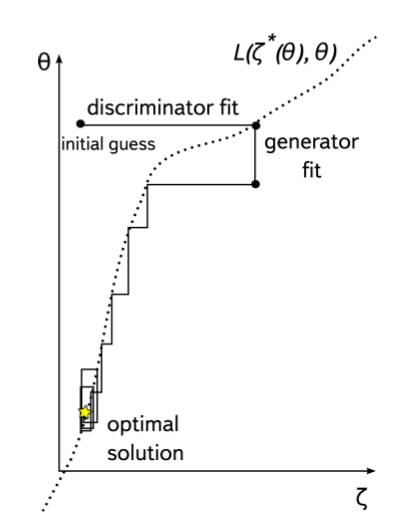
\includegraphics[width=0.4\linewidth]{gan-training}}
			\caption{Схематическое изображение процесса обучения GAN.}
			\label{gan-training}
		\end{figure}
	\subsection{Модификации}
		\subsubsection{pix2pix GAN}
			Для решения задачи было попробовано применить модификацию GAN-сети под названием "pix2pix GAN" \cite{p2p}. Ее отличие от схемы GAN, введенной выше, состоит в том, что вместо шума на вход генератору приходят другие изображения, на которых он основывается при синтезе. Схематически ее устройство изображено на (Рис. \ref{p2p}).
			\begin{figure}
				\centering{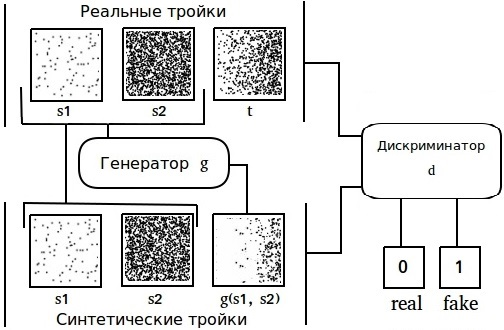
\includegraphics[width=0.65\linewidth]{p2p}}
				\caption{Схематическое устройство сети pix2pix GAN.}
				\label{p2p}
			\end{figure}
			Для pix2pix сети общий функционал потерь выглядит следующим образом: $$ L(G, D) = L_{adv}(G, D) + \eta \mathbb{E}_{p_{data}(s_1, s_2, r)} (\parallel r - G(s_1, s_2) \parallel_1)$$
			$$ L_{adv}(G, D) = \mathbb{E}_{p_{data}(s_1, s_2, r)}\log D(s_1, s_2, r) +  \mathbb{E}_{p_{data}(s_1, s_2)} \log (1 - D(s_1, s_2, G(s_1, s_2)))$$
			где G, D - генератор и дискриминатор, $(s_1, s_2, r)$ - тройка изображений (интенсивность слева, справа и реальное изображение с трендом),  $\mathbb{E}_{p_{data}(s_1, s_2, r)}$ - мат. ожидание логарифмического правдоподобия того, что тройка изображений $(s_1, s_2, r)$ принадлежит вероятностному распределению реальных троек $p_{data}(s_1, s_2, r)$, а $p_{data}(s_1, s_2)$ соответствует распределению реальных изображений $s_1, s_2$.
			\begin{figure}
				\centering{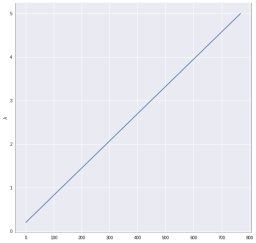
\includegraphics[width=0.75\linewidth]{trend}}
				\caption{Вход и желаемый выход нейросети-генератора.}
				\label{p2p-gen}
			\end{figure}
			\begin{figure}
				\centering{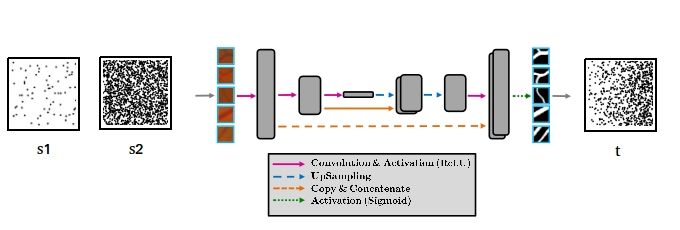
\includegraphics[width=1\linewidth]{unet-scheme}}
				\caption{Схематическое изображение нейросети-генератора.}
				\label{unet-sheme}
			\end{figure}